% Editing? Enable word wrap in your editor.

\documentclass{report}
\usepackage{fullpage}
\usepackage{a4}
\usepackage{geometry}
\usepackage{fancyhdr}
\usepackage{etoolbox}
\usepackage{hyperref}
\usepackage{graphicx,float}
\usepackage{subfig}
\usepackage{array,ragged2e,pst-node,pst-dbicons}
\usepackage{mdframed}
\usepackage{minted}
\usemintedstyle{monokai}
\BeforeBeginEnvironment{minted}{\begin{mdframed}[backgroundcolor=black!90]}
\AfterEndEnvironment{minted}{\end{mdframed}}

\usepackage[backend=biber,
style=numeric,
natbib=true,
sorting=none,
citestyle=authoryear]{biblatex}
\addbibresource{./references.bib}

% Required by OCR
\newcommand{\candidatename}{Rain}
\newcommand{\candidatenumber}{0000}
\newcommand{\centernumber}{000000}
\newcommand{\centername}{Center Name}
\newcommand{\qualification}{H446, 2021}

% Apply headers and footers to every page, including chapter pages
% Required by OCR
\pagestyle{fancy}
\setlength{\headheight}{12pt}
\addtolength{\topmargin}{-11pt}
\patchcmd{\chapter}{\thispagestyle{plain}}{\thispagestyle{fancy}}{}{}
\fancyhead[L]{\candidatename}
\fancyhead[C]{Candidate: \candidatenumber}
\fancyhead[R]{Center: \centernumber}
\fancyfoot[L]{\qualification}
\fancyfoot[C]{}
\fancyfoot[R]{\thepage}

\renewcommand{\familydefault}{\sfdefault} % serif fonts are an eyesore

\title{Intelligent flashcards}
\author {
  \candidatename \\\\
  Candidate: \candidatenumber \\
  Center: \centernumber \\
  \centername \\\\
  \qualification
}

\begin{document}
\raggedbottom
\maketitle
\setcounter{page}{2}
\tableofcontents

\chapter{Analysis}
\section{The Problem}
\paragraph{}
Spaced repetition of bite-sized content has been proven to help commit content to memory. Intelligently spacing content apart further increases people's ability to recall information. Flashcards have long been known to be an effective method to memorise content, but actually using them is cumbersome. For one, having to carry a deck at all times is inconvenient; let alone having to constantly sort and move cards around as you become more and less familiar with the content inside. This is a shame, as managing cards intelligently helps to maximise efficiency in retaining information. 

\paragraph{}
This problem is a good candidate for solving computationally: most people carry around a device capable of accessing the internet at all times (more than are willing to carry several decks of flashcards!). In addition, algorithms can help to categorise content and signal the optimal time to practice something. This project aims to solve both of these problems through an online web application.

\section{The Science}
\paragraph{}
By exploiting the psychological spacing effect, people can learn much more efficiently. Humans find it much easier to recall and apply content that has been spaced across several days and shuffled around, compared to content that has been crammed in a single session. Students that learned content across several days in multiple locations were able to recall up to an additional 4 items on average, compared to those who learned the same content on the same day in one location\footcite{ShufflingMathematicsProblems}.

\section{Existing Solutions}
A few pieces of software have already solved this problem. 

\subsection{Tinycards}
\paragraph{}
Duolingo's Tinycards \footcite{Tinycards} (defunct since September 2020), was likely the closest implementation to what this project aims to achieve. The user could pick one of already created decks of cards containing material they wanted to study, or create their own. Then, the software would present a range of challenges based on how well the user retained the information. 

\begin{figure}[h!]
  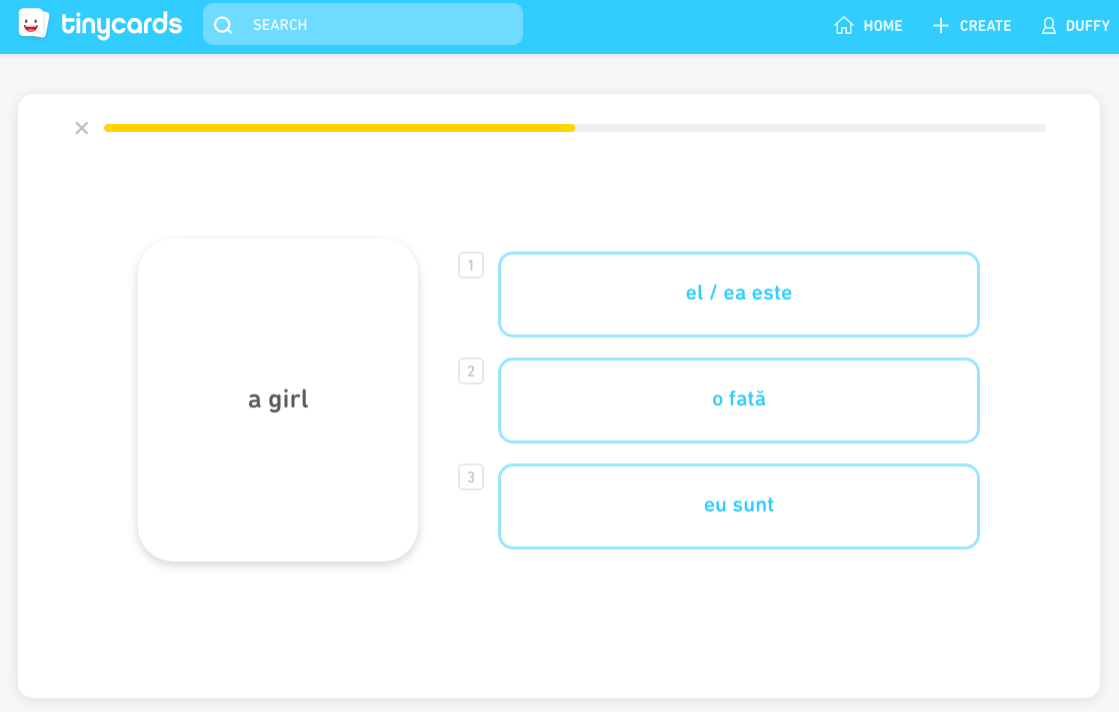
\includegraphics[width=\linewidth]{./media/tinycards.png}
  \label{fig:tinycards1}
  \caption{A screenshot of the desktop user interface for Tinycards. Sourced from \href{https://web.archive.org/web/20211005121604/https://www.pcmag.com/reviews/tinycards-by-duolingo}{PCMag}.}
\end{figure}

\paragraph{}
This ranged from simply showing the card and letting the user get to grips with it; matching one side of the card with another card from a line-up; or typing the other side of the card from memory. The site eventually had to shut down due to lack of financial resources, but not before gaining over 1.5 million active monthly users\footcite{TinycardsShutdown}.

\subsection{Physical Flashcards}
\paragraph{}
Paper flashcards are likely most people's first thought when it comes to spaced-repetition learning. They are simple to understand, and \emph{can} be very effective when paired with a suitable system such as Leitner boxes.

\paragraph{}
Using them effectively, however, is a challenge. Organising many cards is very difficult — not to mention that cards can be damaged or lost. In addition, creating them can be very time-consuming, and many do not know how to use the cards properly to maximise recall once they have been created.

\subsection{Quizlet}
\paragraph{}
Quizlet solves some of these problems by featuring a flashcard mode. However, there is no algorithm to intelligently distribute and challenge cards, like there was in Duolingo's Tinycards. As such, this is little more than a digitised analogue of paper cards. While this is certainly better than having to carry about paper cards, this can absolutely be improved upon with intelligent algorithms.

\section{Stakeholders}

\subsubsection{Students}
\paragraph{}
The main target of this software are students — particularly those at secondary and A-Level. They are the end users, and will make up most interactions. They will use the site to actually learn the content, so it should be intuitive and must meet their needs; the site must effectively help them what they need to learn. Students can be conversed with during or after school hours on most days of the week.

\subsubsection{Teachers}
\paragraph{}
Teachers are also important to consult with, even if they might not directly use the software; being teachers, their job is to ensure that content is taught effectively. They have significant experience and training in effective learning methods, so they are a vital resource in ensuring the efficacy of the software. Time with teachers will be much more restricted, especially as the year progresses towards exam season.

\subsection{Students}
\paragraph{}
Having outlined the issues with existing solutions, interviews with several students were conducted to gather details about what they would need from this piece of software. Some notable excerpts are listed below. Names have been reduced to initials.

\hrulefill
% --------------------------------------
\subsubsection{How often do you revise?}
\begin{quote}{Student J:}
  Never; well, not really. When I say "never", I mean right before like a test or something.
\end{quote}

\begin{quote}{Student U:}
  Every two days.
\end{quote}
% --------------------------------------
\subsubsection{What methods do you use for revision?}
\begin{quote}{Student J:}
  \href{https://senecalearning.com/en-GB/}{Seneca}; It's easy to use and requires little input. If I'm deciding what questions I'm revising, I might not know what's gonna be on the test. Seneca has the content that I need.
\end{quote}

\begin{quote}{Student U:}
  Mainly reading textbooks and exam questions.
\end{quote}
% --------------------------------------
\subsubsection{What features would you look for in a revision tool?}
\begin{quote}{Student J:}
  Ideally, it gives me the questions that I don't know the best. Covers all the topics, obviously. The questions aren't asking me to repeat what I've just read. I hate that [about Seneca].
\end{quote}

% --------------------------------------
\subsubsection{What keeps you from revising as much as you should / revising more often?}
\begin{quote}{Student J:}
  We live in a golden age of television and gaming. [Revision is boring by comparison.]
\end{quote}

\begin{quote}{Student U:}
  Boredom.
\end{quote}
% --------------------------------------
\hrulefill

\paragraph{}
Note that while Student U revises often, the way they revise doesn't help to practice the skills they need. Their revision is passive (i.e. reading from a textbook) instead of active (e.g. answering recall and practice questions). Meanwhile, Student J uses active revision methods, but has not formed a routine around it.

\paragraph{}
In summary, students want a tool that is engaging and fun. More importantly, it must have the content that they need and present the information realistically. It should also help to build habits to ensure effectiveness.

\subsection{Teachers}
\paragraph{}
// Todo

\section{Requirements}
\paragraph{}
Based on the thoughts of the stakeholders, the following requirements were drawn up.

\subsection{Authentication}
Being able to target individual users allows for personalised learning. This means that there has to be a way for each user to be uniquely identified.
\begin{itemize}
  \item Must have a registration page:
  \begin{itemize}
    \item Take username and password.
    \item Password must be typed twice to prevent mistakes, and be masked to prevent shoulder surfing.
    \item Prevent automated registration attempts, such as through a captcha.
    \item Optionally allow the user to use 2FA.
  \end{itemize}
  \item Must have a sign-in page:
  \begin{itemize}
    \item Sign in must be rate-limited to prevent automated attempts.
    \item Sign in must be protected by captcha to prevent automated attempts.
  \end{itemize}
\end{itemize}

\subsection{Feel and branding}
The software should feel friendly, familiar, casual and playful. One of the most oft cited reasons for avoiding revision is that it is boring compared to other things that they could be doing.
\begin{itemize}
  \item Interface should be simple, uncluttered and clean.
  \begin{itemize}
    \item Interface should be as simple as possible. Nothing should be redundant. Prefer icons to text.
    \item Interface should put the content front and centre and minimise distractions.
    \item Interface should feature a dark theme, which may be more comfortable in some lighting conditions.
    \item Interface should be accessible to those who are colour-blind (1 in 12 men are colour-blind\footcite{Colourblindness}).
  \end{itemize}
  \item Branding should be casual and playful.
\end{itemize}

\subsection{Decks and Cards}
Cards are the focus of the app, and what the user will spend most time interacting with.
\begin{itemize}
  \item Users can create their own cards and decks.
  \begin{itemize}
    \item Users edit the front and back of their cards.
    \item Users can choose to share their decks with other users.
    \item Users can tag their decks, e.g. by subject / topic.
  \end{itemize}
  \item Users can search a list of public decks.
  \begin{itemize}
    \item A fuzzy search feature searches decks, the cards inside the deck, and the tags of the cards.
    \item Users can import other users' decks to practice or edit their own copy.
  \end{itemize}
  \item Users are shown and tested on their decks. Algorithms figure out how well a user knows a card, and might present the card in different ways depending on how familiar the user is.
  \begin{itemize}
    \item Presented with the card to read and nothing else.
    \item Presented with a card and asked to pick the other side from a line-up of several cards.
    \item Presented with a card and then asked to type out the other side from memory.
    \begin{itemize}
      \item The checking mechanism should be fuzzy and lenient to typos or alternative phrasing. This might be accomplished through an algorithm like Levenshtein edit distance.
      \item The software should allow a user to mark a question that has been judged incorrect as being correct. For example, this might be because of alternative phrasing that throws off edit distances.
    \end{itemize}
  \end{itemize}
  \item The user is offered some sort of incentive to come back every day to practice.
  \begin{itemize}
    \item This could be accomplished through things like daily streaks on decks, graphs of performance and a daily challenge.
  \end{itemize}
\end{itemize}

\subsection{Moderation}
The site is public with anyone being able to submit public cards. There needs to be a way to ensure that public cards are appropriate.

\begin{itemize}
  \item Decks marked as forkable (i.e. public) can be flagged by users for review by a moderator.
  \begin{itemize}
    \item The offending card can be deleted by a moderator.
    \item The offending user can be banned by a moderator.
  \end{itemize} 
\end{itemize}

\section{Success criteria}
\subsection{Backend}
\paragraph{}
The backend should satisfy all the requirements listed above. Furthermore, it should be secure against common exploits such as SQL injection to prevent leaking or destruction of user data. The backend should be able to run on any server machine in a portable manner, allowing for easy deployment and self-hosting, should users choose to do so. The backend should be thoroughly tested, perhaps using an automated testing engine. We can generate code coverage reports from our testing engine to view the effectiveness of our tests.

\subsection{Frontend}
\paragraph{}
The frontend should be responsive to many viewport sizes, be accessible, load quickly on slow connections and stay performant even on lower end hardware, as might be typical on a student's device. We can generate scores for these metrics using Google's Lighthouse, a web auditing tool that reports on important metrics that affect perceived and actual performance, as well as highlighting any accessibility issues. Lighthouse was chosen as it is an industry standard testing tool, and the Google search engine considers Lighthouse scores when ranking pages in its search results. At a minimum, we should strive for a score of 90 or higher in every category.

\paragraph{}
We can also end-to-end test the user interface using both automated means to iron out any bugs, and with users to locate any UX issues. We can measure this by having in person tests with users of the target demographic (13-21 year olds) and seeing how they interact with the software, measuring time it takes to do certain tasks and asking them to describe their experience and any pain points with the software.

\chapter{Design}
\paragraph{}
The software can be broken down like so:

\begin{itemize}
  \item User \begin{itemize}
    \item Decks \begin{itemize}
      \item Cards \begin{itemize}
        \item Front
        \item Back
        \item Ability history
        \item Metadata, e.g. owner, forkable.
      \end{itemize}
    \end{itemize}
    \item Account info \begin{itemize}
      \item Username
      \item Password hash
      \item Session tokens
    \end{itemize}
  \end{itemize}
\end{itemize}

\paragraph{}
Everything is tied to each user. The user can create their own decks and cards, and share them with other users. Each deck can be tagged with a subject or topic, allowing for easy searching if they choose to make these decks public.

\section{Paradigm and architecture}
\paragraph{}
A website allows the software to target the largest amount of devices with the least effort. However, this has the downside of requiring stable internet access, which is not always available.

\paragraph{}
Originally, an object-oriented approach was considered. However, this does not make a lot of sense for this project. To ensure maintainability, scalability, and open up the possibility for development of mobile apps in future, a RESTful design was chosen for the backend. Because of this, each request does not leave behind persistent state in the server memory (i.e. it is stateless). As such, constructing instances of classes for each request just to be destroyed at the end of the request is not a good idea. A functional approach supports this architecture much better.

\paragraph{}
The user interface should be divorced from backend logic, similar to a "JAM-stack". This allows it to be deployed to a CDN for low latency globally, reducing hosting costs, and once again keeping the door open for dedicated mobile applications.

\section{Database design}

\begin{figure}[h!]
  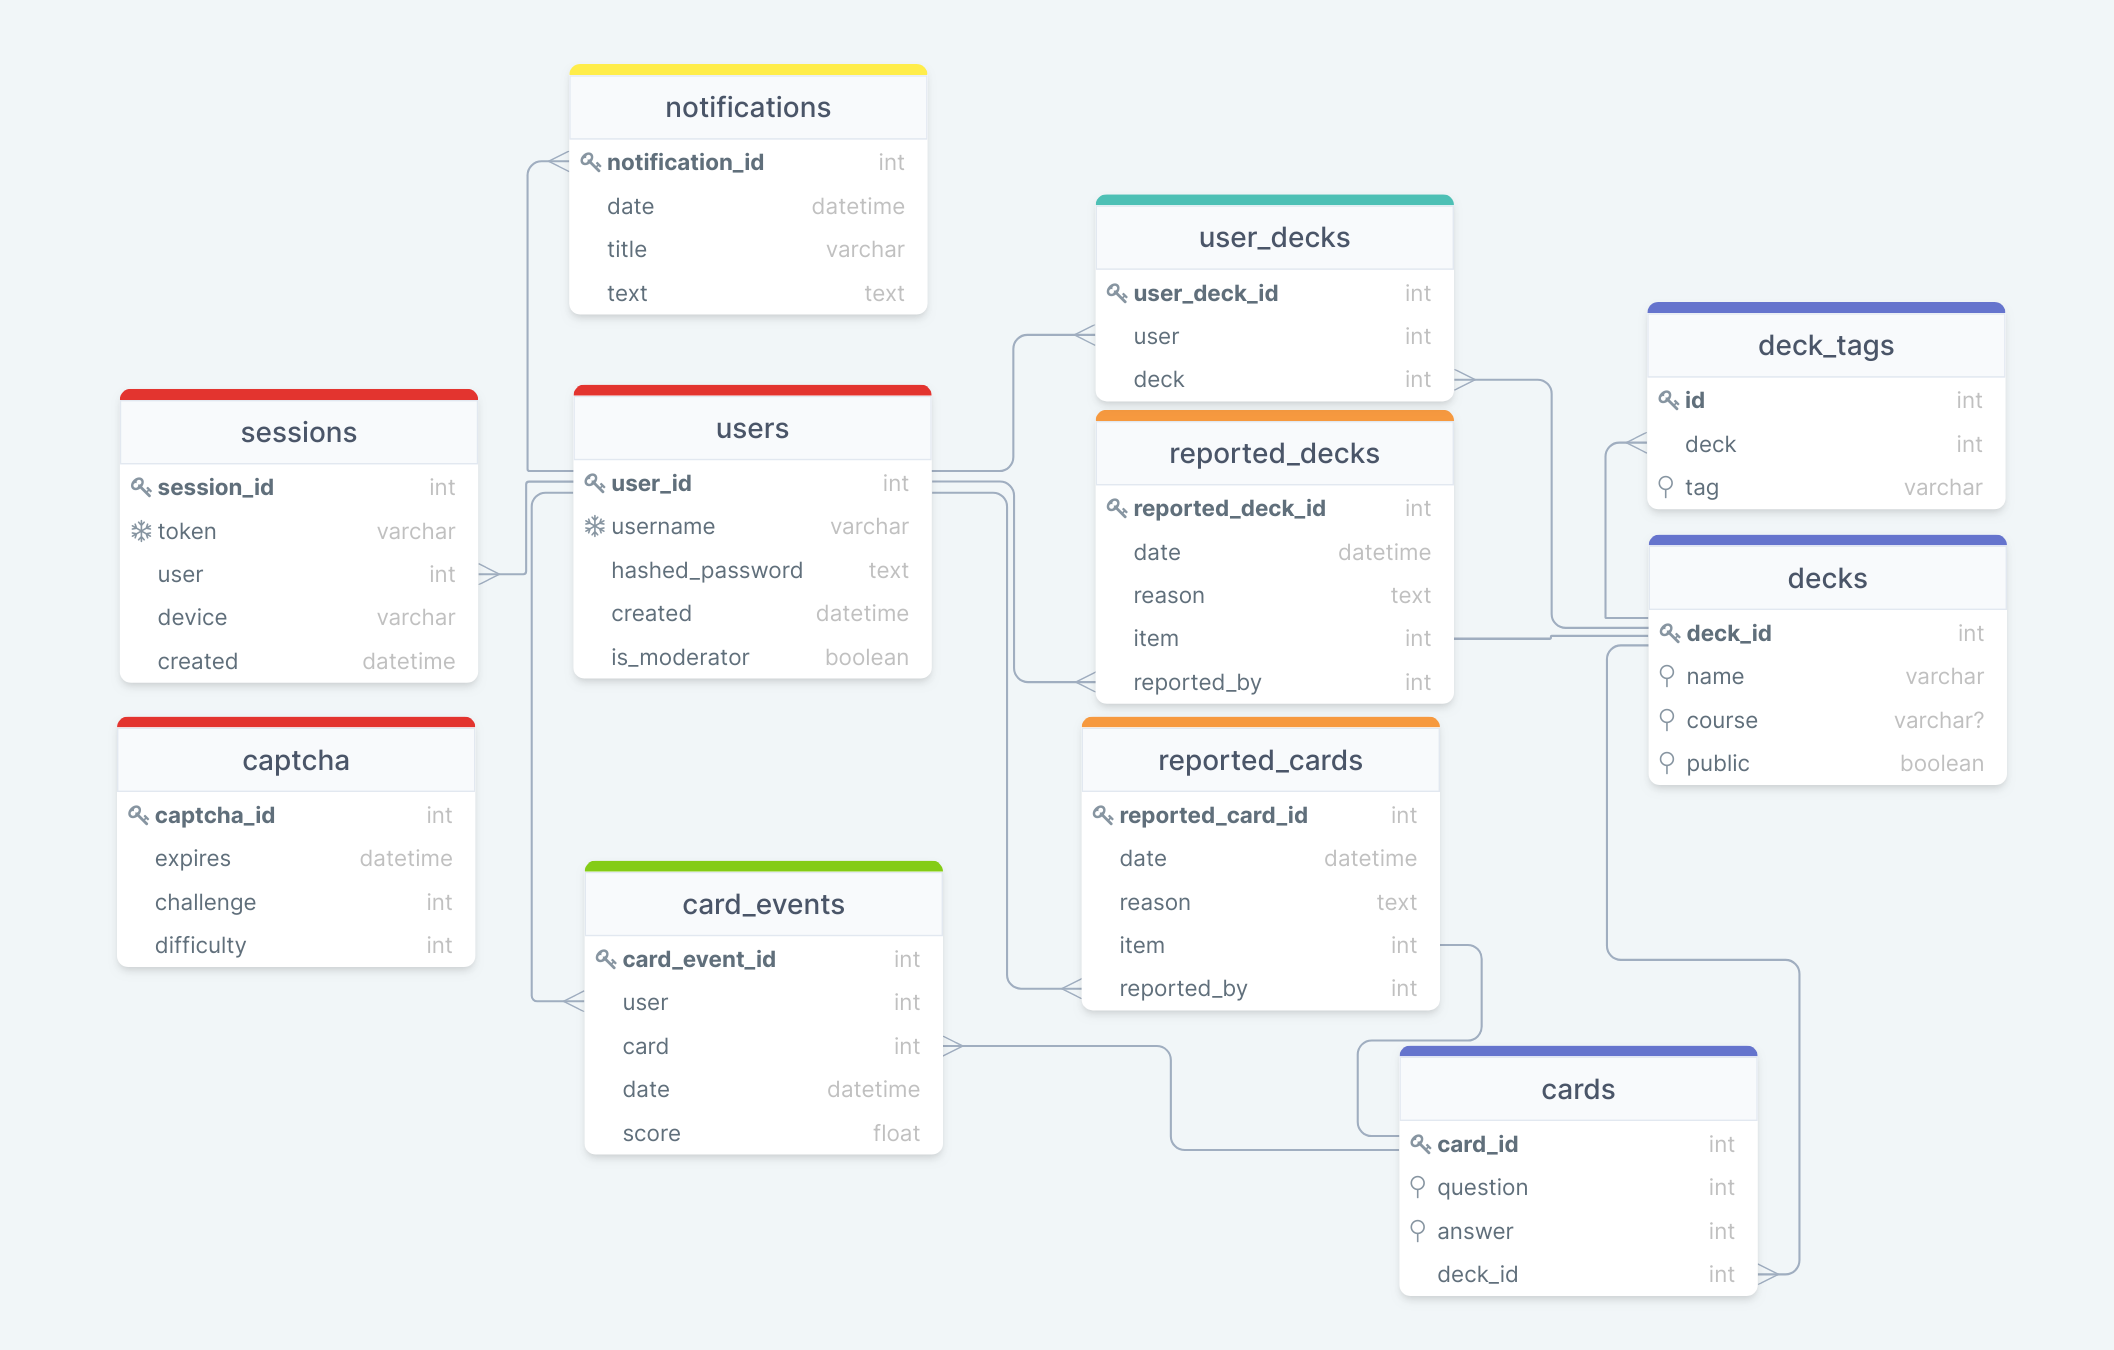
\includegraphics[width=\linewidth]{./media/db_schema.png}
  \label{fig:database1}
  \caption{Database schema. \href{https://drawsql.app/--347/diagrams/iroase}{Click here} to see a scalable diagram.}
\end{figure}

\paragraph{}
Users have many decks, which can hold many cards. Originally, a NoSQL document-driven database like MongoDB was going to be used, but due to the common request of wanting to share decks, a relational SQL database will be more suitable. These complex relationships would need multiple transactions in a NoSQL database, while a relational database is much more suitable as it can easily deal with complex, interconnected data in a single transaction. A search system could be implemented on cards that users have marked as forkable to allow users to adopt a copy of other decks to their account. This search feature could index cards based on keywords and exam boards.

\paragraph{}
Storing authorization info allows users to be remembered by the site. Storing the password in hashed form allows the user to be protected in case of database breaches, and salting the hash further prevents the use of rainbow tables.

\paragraph{}
Reports need to be saved to keep the site safe from spam or harmful content. These reports can then be reviewed by a moderator.

\paragraph{}
CardEvent is used to track the user's ability to remember cards. This can then be used to calculate how well a user knows a card.

\paragraph{}
Notifications are stored in the database, so the user can be told about important events such as a card they have reported has being checked by a moderator.

\subsection{Data flow}
\paragraph{}
A user signs up through the frontend, which saves their username and a salted hash of their password into the Users table. A user can then create a deck, which creates a deck in the Decks table, with a reference to their deck in UserDecks. They can then create cards, which creates cards in the Cards table, with a reference to their deck in UserDecks. Cards can be created, with a reference to their deck in DeckCards. Once a user begins using their decks, the software can then calculate the ability of the user to remember each card and store it in the database based on a "confidence" score and a date. Storing this information allows for an algorithm similar to Leitner boxes to be used to serve cards at optimal intervals. This cycle of reviewing cards repeatedly makes up the core functionality of the software.

\paragraph{}
If a user wants to share their deck with other users, they can mark it as public. This allows it to be returned in search results, and for other users to adopt a copy to their account for them to then use in a similar fashion.

\section{Algorithms}
\subsection{Calculating pull rate}
\paragraph{}
Cards that have high fluctuations of confidence are more difficult to remember, and cards that have low fluctuations are easier to remember.
\paragraph{}
We can represent this mathematically. $0 \leq c < 1$ represents the confidence ($c$) of the card, where $c = 0$ means the card is completely forgotten, and $c = 1$ means the card is completely remembered. 

\paragraph{}
Humans do not remember things linearly, however\footcite{ForgettingCurve}. There is a sharp decline in retention just one day after learning it. This is because it has not been shifted to long term memory. Because of this, a linear equation can't be used to judge the ability of a user to remember a card. 

\paragraph{}
Suppose we have a user that practices a card once. We can model how the card might decay in their memory against time in days passed since review ($t$) with this equation:
\[
  y = \frac{1}{(t + 1) ^ {2}}
\]

\paragraph{}
We need to account for this decay in confidence by pulling poorly remembered cards more often than well remembered cards, while also considering time. If we can delay reviews such that the review happens right before forgetting a card, we can maximise the boost in confidence.

\paragraph{}
We can define forgetting a card as a sudden decrease in confidence at a review ($\Delta c < -0.4$), or number of times confidence  has gone below a certain threshold ($c < 0.15$). This value can be $f$, for the number of times the card has been forgotten.

\paragraph{}
Bringing this all together, we end up with a way to rank the order the cards should be pulled, with $P$ being the "Pull" value.

\[
  P = \frac{1}{(t + 1) ^ 2} \cdot \frac{n}{c ^ {-1}} \cdot \frac{1}{f + 1}
\]

$n$ represents the number of days on which the card has been reviewed.

$t$ represents an amount of time since the card was last reviewed.

$f$ represents the number of times the card has been forgotten.

Cards with a lower value of $P$ should be pulled first.

\paragraph{}
The $\frac{1}{(t + 1) ^{2}}$ term is used to model memory decay over time, with higher values of $t$ reducing the value of $P$.

\paragraph{}
The $\frac{n}{c ^{-1}}$ term is used to model the ability of the user to remember the card. A higher value of $n$ (more reviews) against a lower value of $c$ (low confidence) significantly decreases the value of $P$, as the card is likely very difficult.

\paragraph{}
The $\frac{1}{f + 1}$ term is used to model the number of times the card has been forgotten. A lower value of $f$ increases the value of $P$.

\paragraph{}
More concretely, suppose a user has a card, $A$, that they are very familiar with ($c = 0.85$). They have never forgotten it ($f = 0$), and have been doing reviews on it on ten different days ($n = 10$), with the last review being 30 hours ago ($t = 30$) We can calculate the following:

\[
  P _ A = \frac{1}{(30 + 1) ^ 2} \cdot \frac{10}{0.85 ^ {-1}} \cdot \frac{1}{0 + 1}
\]

\[
  P _ A = \frac{1}{(31) ^ 2} \cdot \frac{10}{0.85 ^ {-1}}
\]

\[
  P _ A = \frac{1}{961} \cdot \frac{10}{0.85 ^ {-1}}
\]

\[
  P _ A = \frac{17}{1922} = 0.008844953174
\]

\paragraph{}
Now suppose a user has a card, $B$, that is very difficult to remember ($c = 0.04$).  They keep forgetting it ($f = 8$), and have been doing reviews on it on ten different days ($n = 10$), with the last review being 60 hours ago ($t = 60$). We can calculate the following:

\[
  P _ B = \frac{1}{(60 + 1) ^ 2} \cdot \frac{10}{0.04 ^ {-1}} \cdot \frac{1}{8 + 1}
\]

\[
  P _ B = \frac{1}{(61) ^ 2} \cdot \frac{10}{0.04 ^ {-1}} \cdot \frac{1}{9}
\]

\[
  P _ B = \frac{1}{3721} \cdot \frac{10}{0.04 ^ {-1}} \cdot \frac{1}{9}
\]

\[
  P _ B = \frac{2}{167445} = 0.00001194422049
\]

\[
  P _ B < P _ A
\]

As expected, the harder card $B$ results in a lower Pull value, so should be selected first.

\paragraph{}
If we create a new card, $C$, that has never been reviewed ($t = 0, f = 0, n = 0, c = 0$), we end up with an equation that reduces to this:

\[
P _ C = \frac{0}{0 ^ {-1}}
\]

$0 ^ {-1}$ is undefined, so the result of this is undefined. However, we can treat this as a Pull value of $0$ for our purposes, mathematicians be damned. In other words, this card has the highest priority for our algorithm. In the event of a tie because of this rule, we simply choose a random card from the tied cards.

\subsection{Challenge types}
\paragraph{}
Now that we have a way to determine the Pull value of a card, we can start to decide what kind of challenges to serve the user once the card has been pulled. These challenges consider the confidence level of the card. 

\subsubsection{Confidence thresholds}
\paragraph{}
$0 \leq c < \frac{1}{3}$ is a low confidence card, so we serve a "challenge" that simply asks the user to review the card and rate it. We update the confidence accordingly based on if the user finds the card easy, medium, or hard.

\paragraph{}
$\frac{1}{3} \leq c < \frac{2}{3}$ is a medium confidence card, so we serve a challenge that asks the user to pick out the other side of the card from a selection of multiple possibilities. Based on how long it takes the user to select the correct card, we update the confidence value, with faster response times meaning higher confidence.

\paragraph{}
$\frac{2}{3} \leq c < 1$ is a high confidence card, so we serve a challenge that asks them to type out the other side of the card from memory. If correct, confidence increases and if incorrect, confidence decreases.

\paragraph{}
Using these thresholds, we can have a variety of challenge types that scale to the user's ability.

\subsection{Captcha}
\paragraph{}
In order to protect against bots, we can require access to certain API endpoints (e.g. registration, sign in, reporting items) require a captcha to be solved. However, traditional captchas result in poor UX and are difficult to solve for able-bodied, able-minded users (let alone those with disabilities), yet are becoming quite easy to solve for advanced bots.

\paragraph{}
We can use an invisible, proof-of-work captcha to solve this problem. Proof of work challenges don't aim to separate bots from humans but instead exist to increase the amount of computational effort it takes to submit a request to the point where it is not worth sending automated requests.

\paragraph{}
Similar to proof of work algorithms used by some cryptocurrencies, we can send a challenge that requires the client machine to brute-force a hash with a desired property, such as a certain amount of leading zeros in the binary digest of the hash.

\paragraph{}
Implementations of this kind of challenge already exist and are being used somewhat commonly on the internet. The most prolific example is \href{https://friendlycaptcha.com/}{FriendlyCaptcha}.

\paragraph{}
We can generate a challenge (such as a random string) on the server and send it to the client. The client would then use a hashing algorithm to repeatedly hash the challenge prepended with its own generated string until it finds a hash that meets the desired property, e.g. starting with 10 zeros. The client then sends the generated string that resulted in the passing hash to the server alongside its request to whatever endpoint the client is trying to access. The server verifies if the solution is correct: if it is, the server services the request.

\paragraph{}
The benefits to this approach are significant compared to a traditional text transcription or image labelling task like Google's reCAPTCHA. For one, reCAPTCHA is very expensive at 1 USD per 1,000 requests. In addition, Google uses reCAPTCHA to track users across the internet, so there are privacy implications for using reCAPTCHA. Further, reCAPTCHA has already been broken with \href{https://2captcha.com/}{services that exist allowing you to pay for a human to solve the challenge for you}. The greatest upside, however, is the complete elimination of friction from legitimate users.

\subsection{Authentication}
Log in and sign up needs to be protected by a captcha.

\subsubsection{Sign up}
\paragraph{}
On sign up, users are asked to send a username they want alongside their password to the server. First, it must check that the username is valid (alphanumeric and within a certain length constraint). If it is valid, the server then checks the database to see if the username is already taken. If it isn't taken, we hash their password with a salt, create a new entry in the Users table with their username, hashed password, salt, the current time. We create a session token and then send the token to the client. If the username is invalid or has already been taken, we send an error back to the client.

\subsubsection{Login}
\paragraph{}
On sign up, users enter their username and password. This is sent to the server, which retrieves the hash and salt from the database. We hash the password with the salt and then compare the hash to the stored hash. If they match, the password is correct and we can create a session to send to the client. If either the username or the password is incorrect, we send an error to the client stating that the username or password is incorrect.

\subsection{Sessions}
Session tokens are symmetrical on the client and the server. The session token should be sent in Authorization header on almost every request. If the token is invalid or missing, we return a 401 Unauthorized.

\section{Frontend}
\subsection{Styles, feel and branding}
\paragraph{}
The app should be intuitive, casual and approachable, but still have some personality. A quirky yet casual feeling style was chosen to help users feel like they are "at home". Mock-up UI screens were created with Figma, and some are in the figures below. See \href{https://www.figma.com/file/7vs7errfunZKlr1wT6j52Z/faded}{this Figma sketch} for scalable versions of all the screens.

\begin{figure}[H]
  \centering
  \subfloat{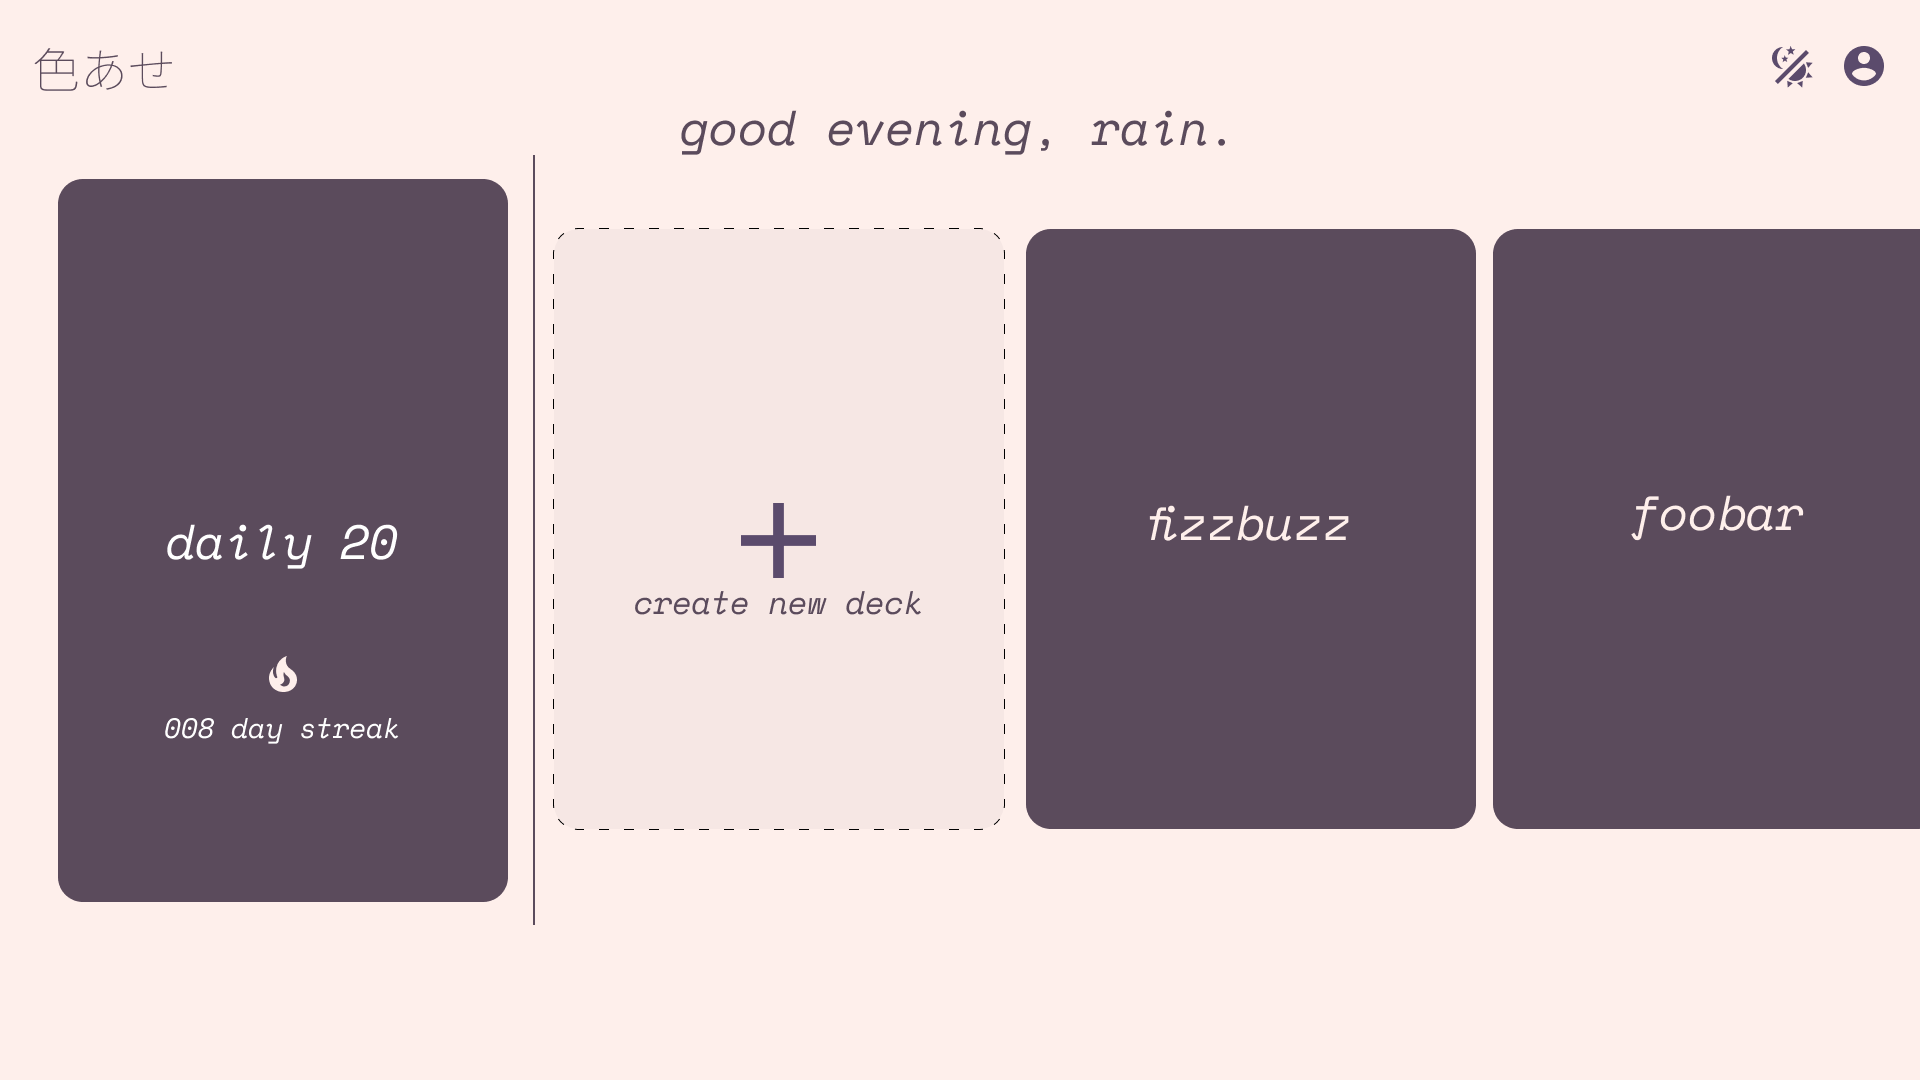
\includegraphics[height=4.2cm]{./media/ui/home.png}}
  \subfloat{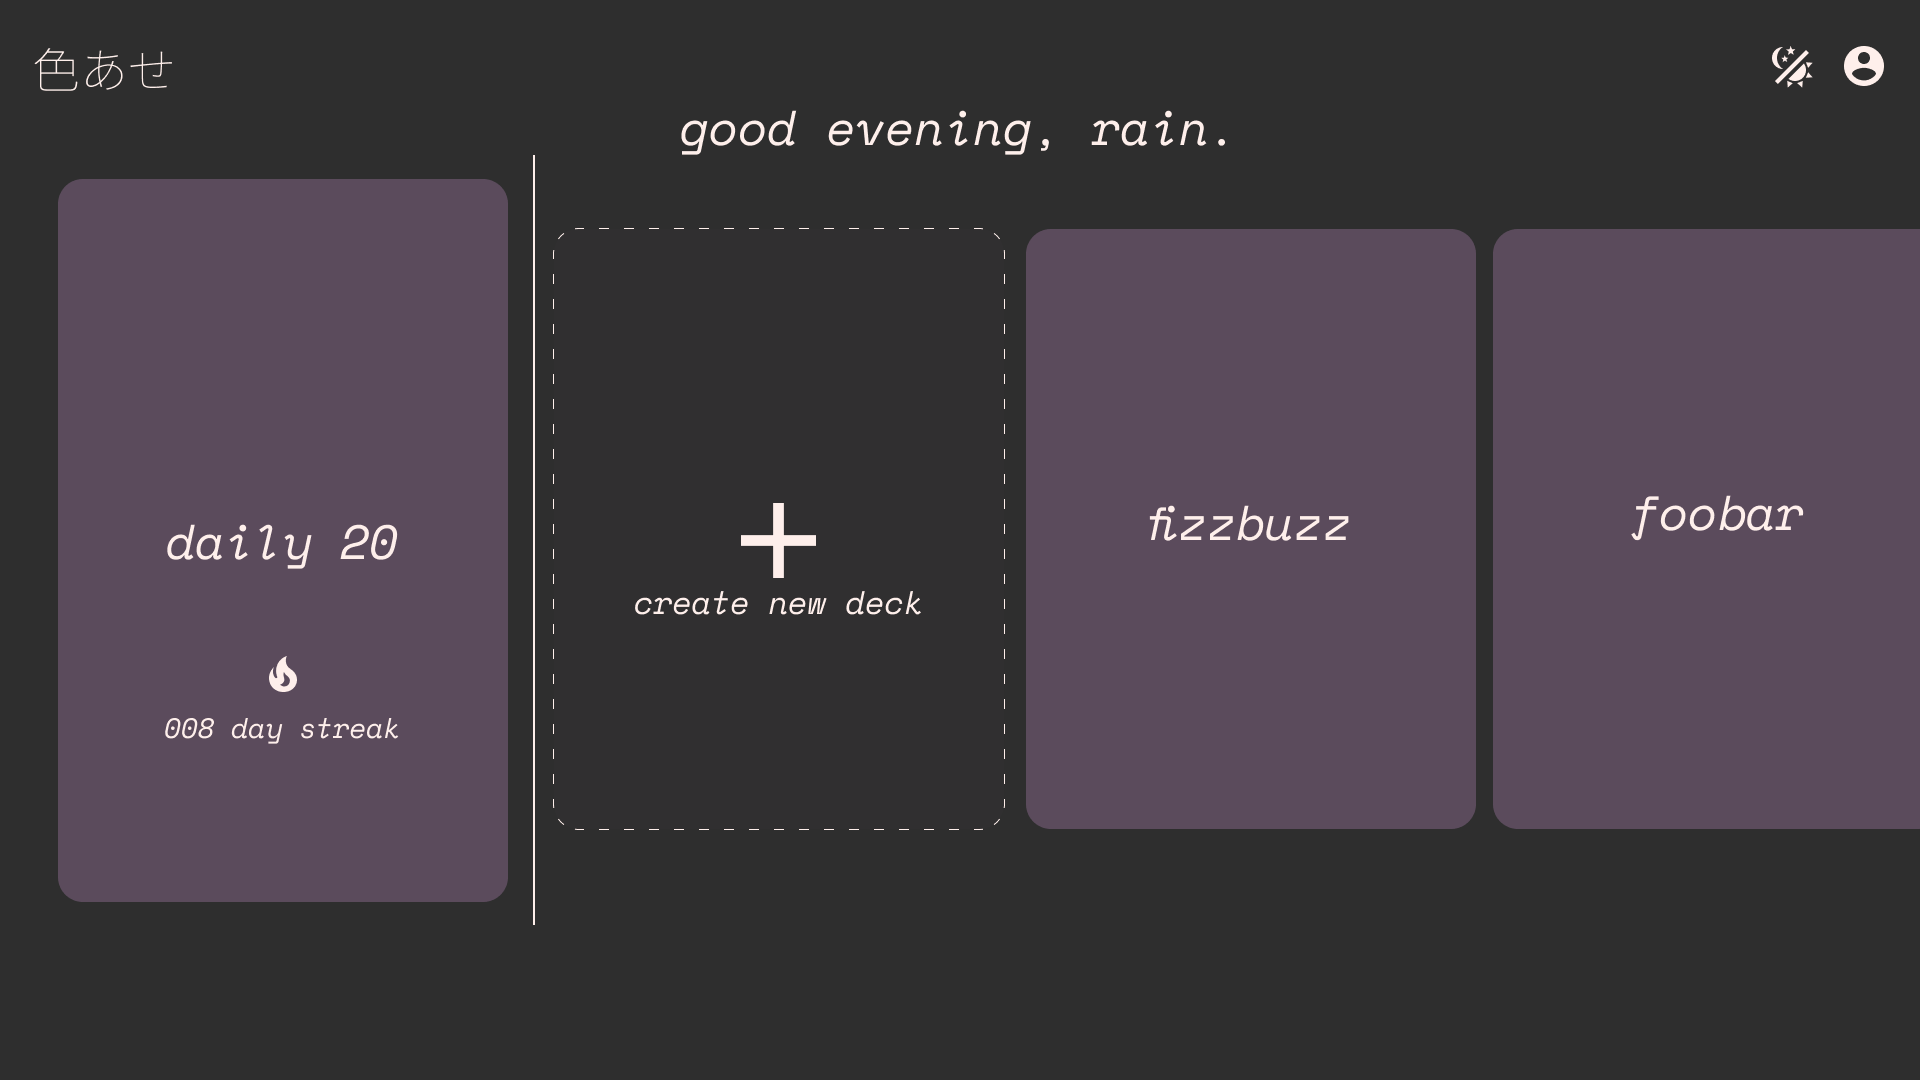
\includegraphics[height=4.2cm]{./media/ui/home_dark.png}}
  \label{fig:home1}
  \caption{The home screen. Text is intentionally lowercase to feel casual; as if the user were typing to friends. A warm colour scheme and a quirky font further makes the site feel less like a sterile textbook. UI components like the navigation bar and cards are as minimal as possible, with further context being revealed on hover. The most important component (daily review) is the largest and separated with a line to hint to the user that is the most important. A streak is shown to motivate the user to practice every day, similar to some social media apps using streaks to encourage daily activity. Dark theme is also available for comfortable reading in low light conditions.}
\end{figure}
\begin{figure}[H]
  \centering
  \subfloat{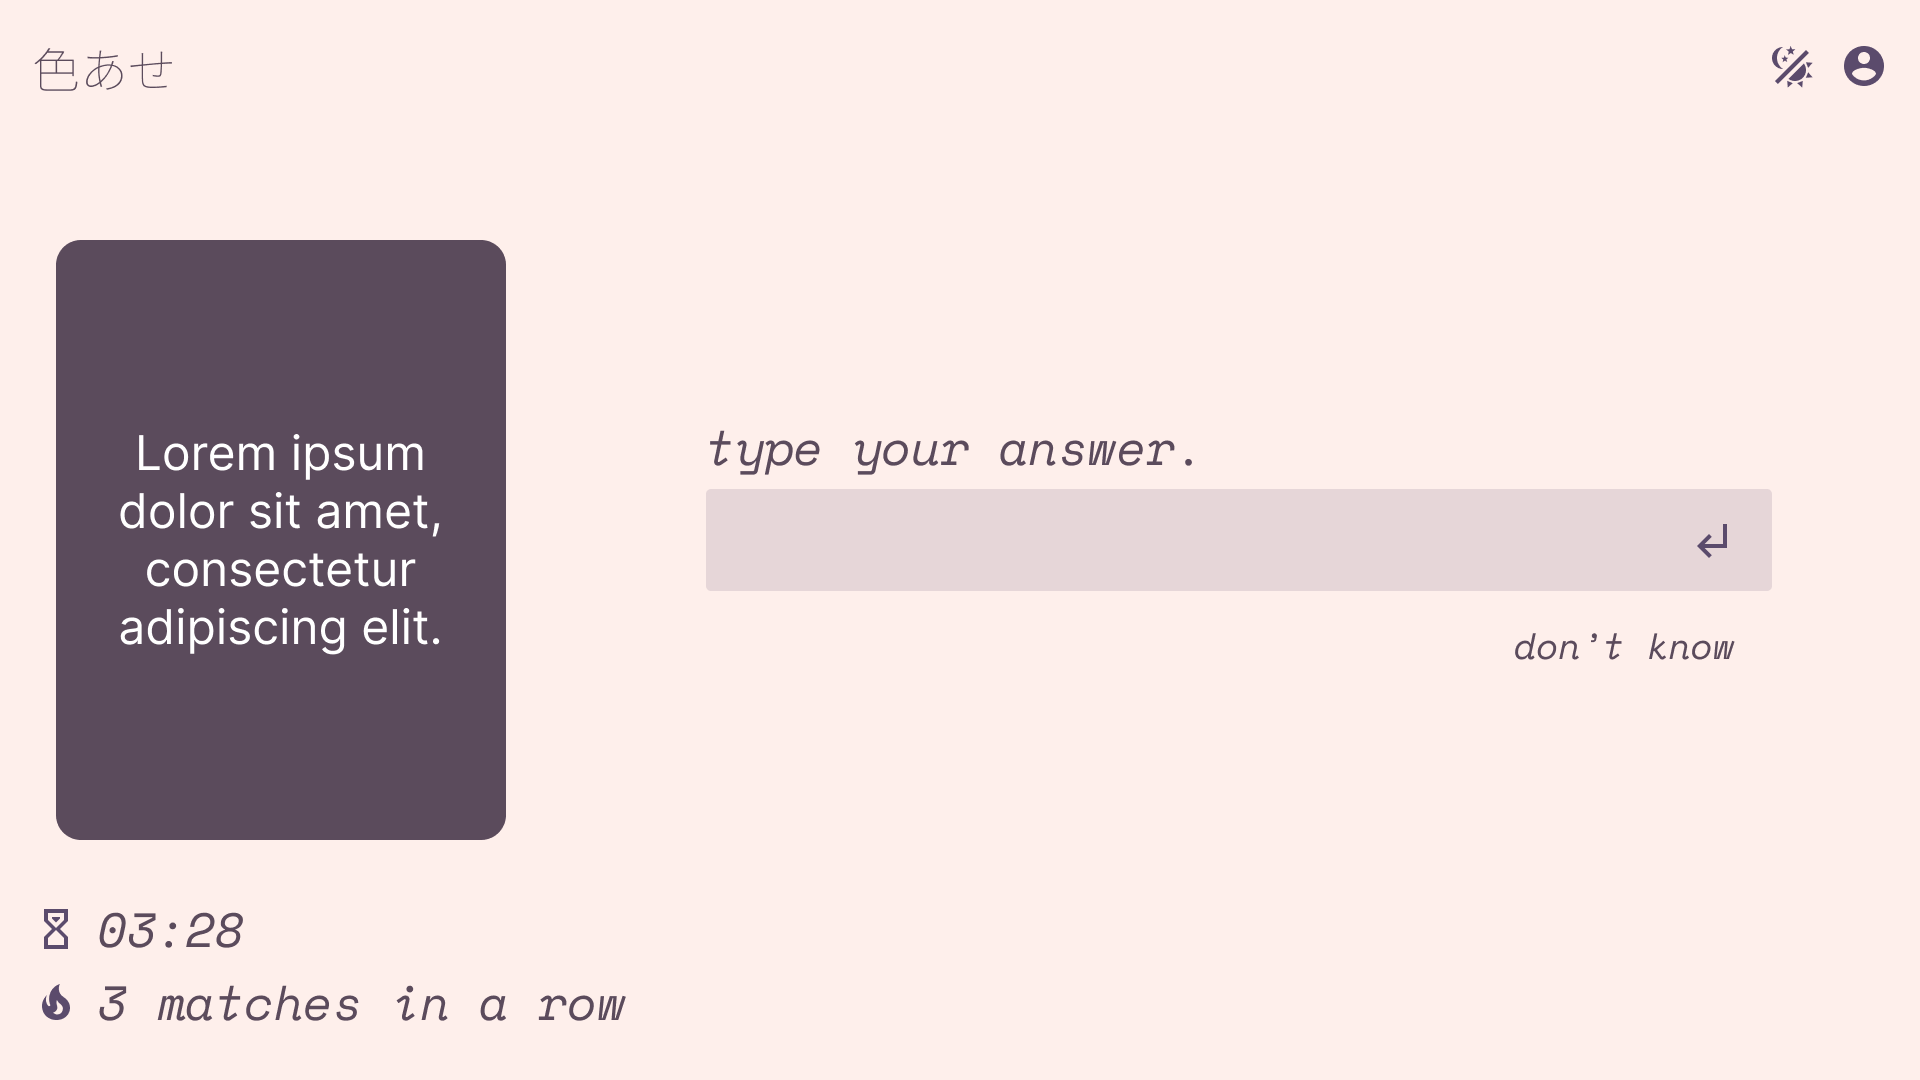
\includegraphics[height=4.2cm]{./media/ui/textbox.png}}
  \subfloat{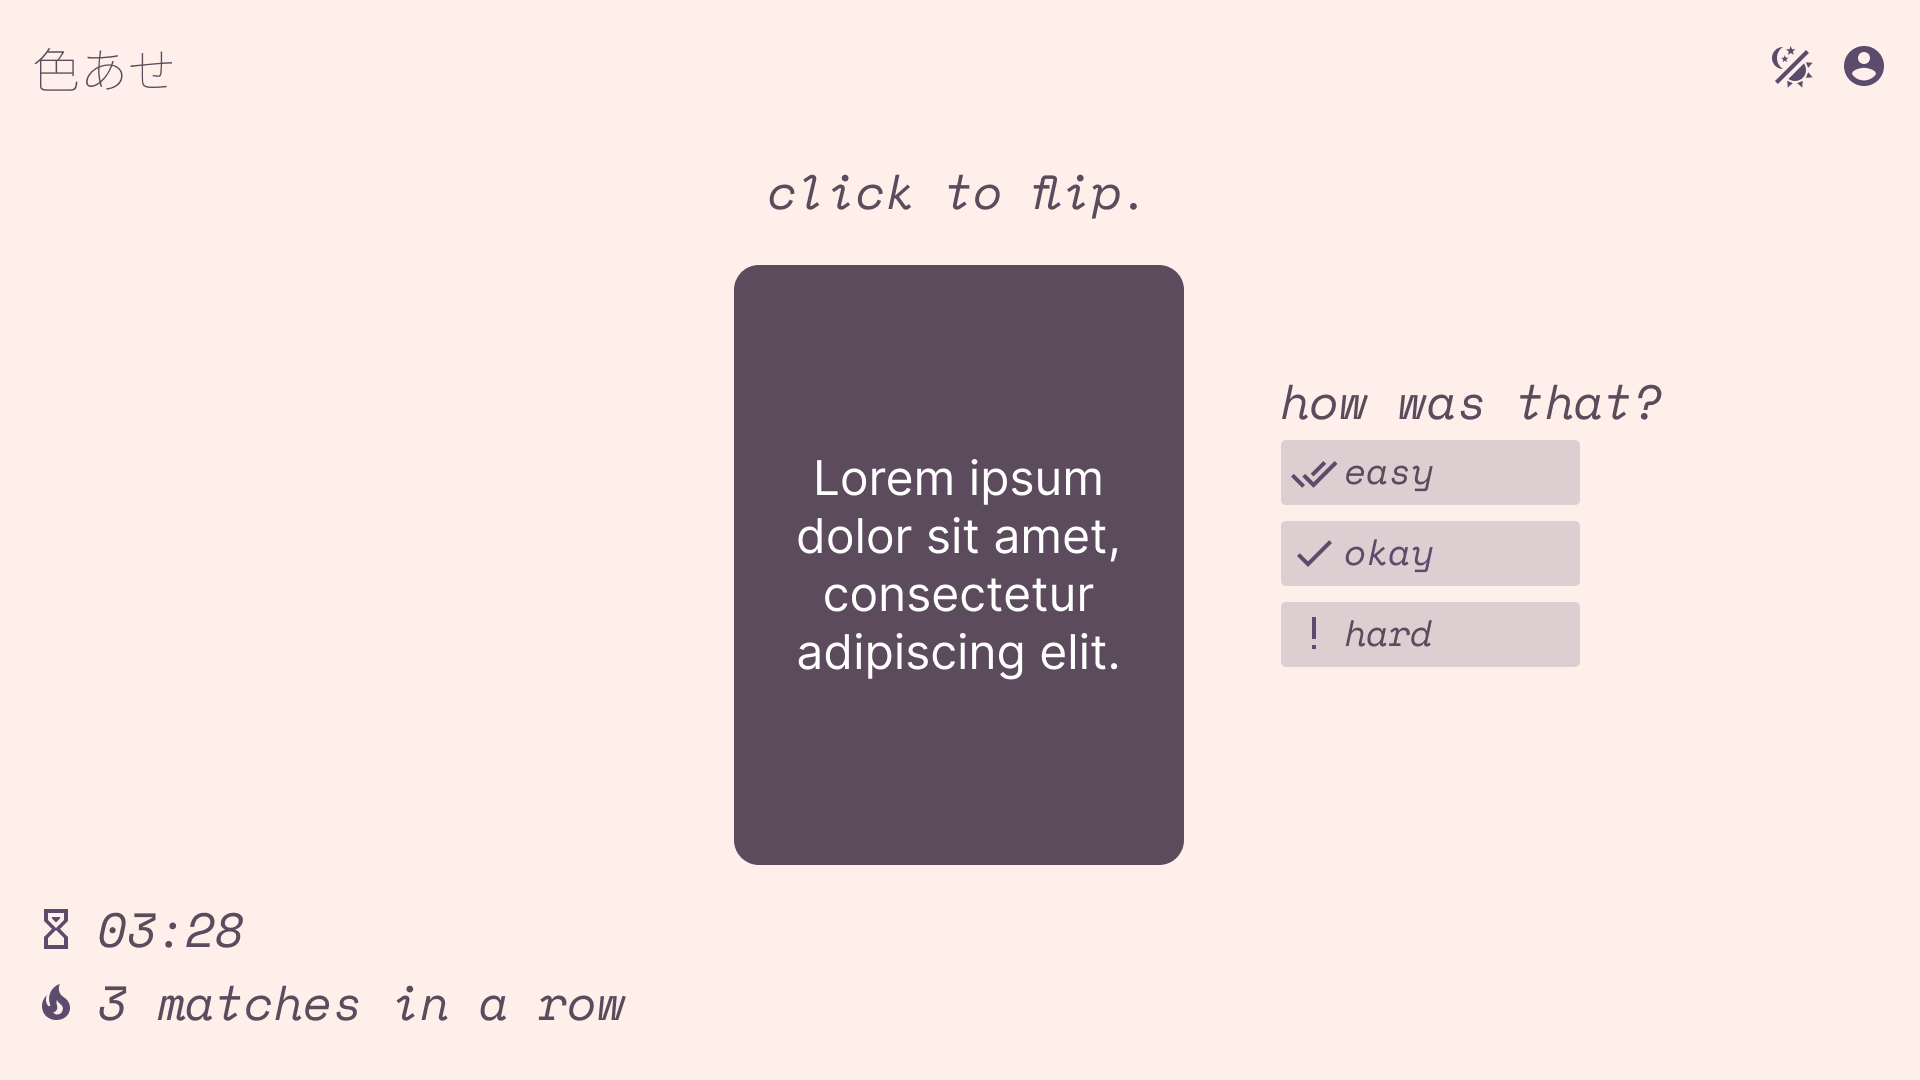
\includegraphics[height=4.2cm]{./media/ui/review.png}}
  \label{fig:question1}
  \caption{Example question screens. A legible, clean sans-serif font with "correct" casing is used on material that is being learned to maximise legibility. Almost nothing else is on-screen, keeping the user focused.}
\end{figure}

\begin{figure}[H]
  \centering
  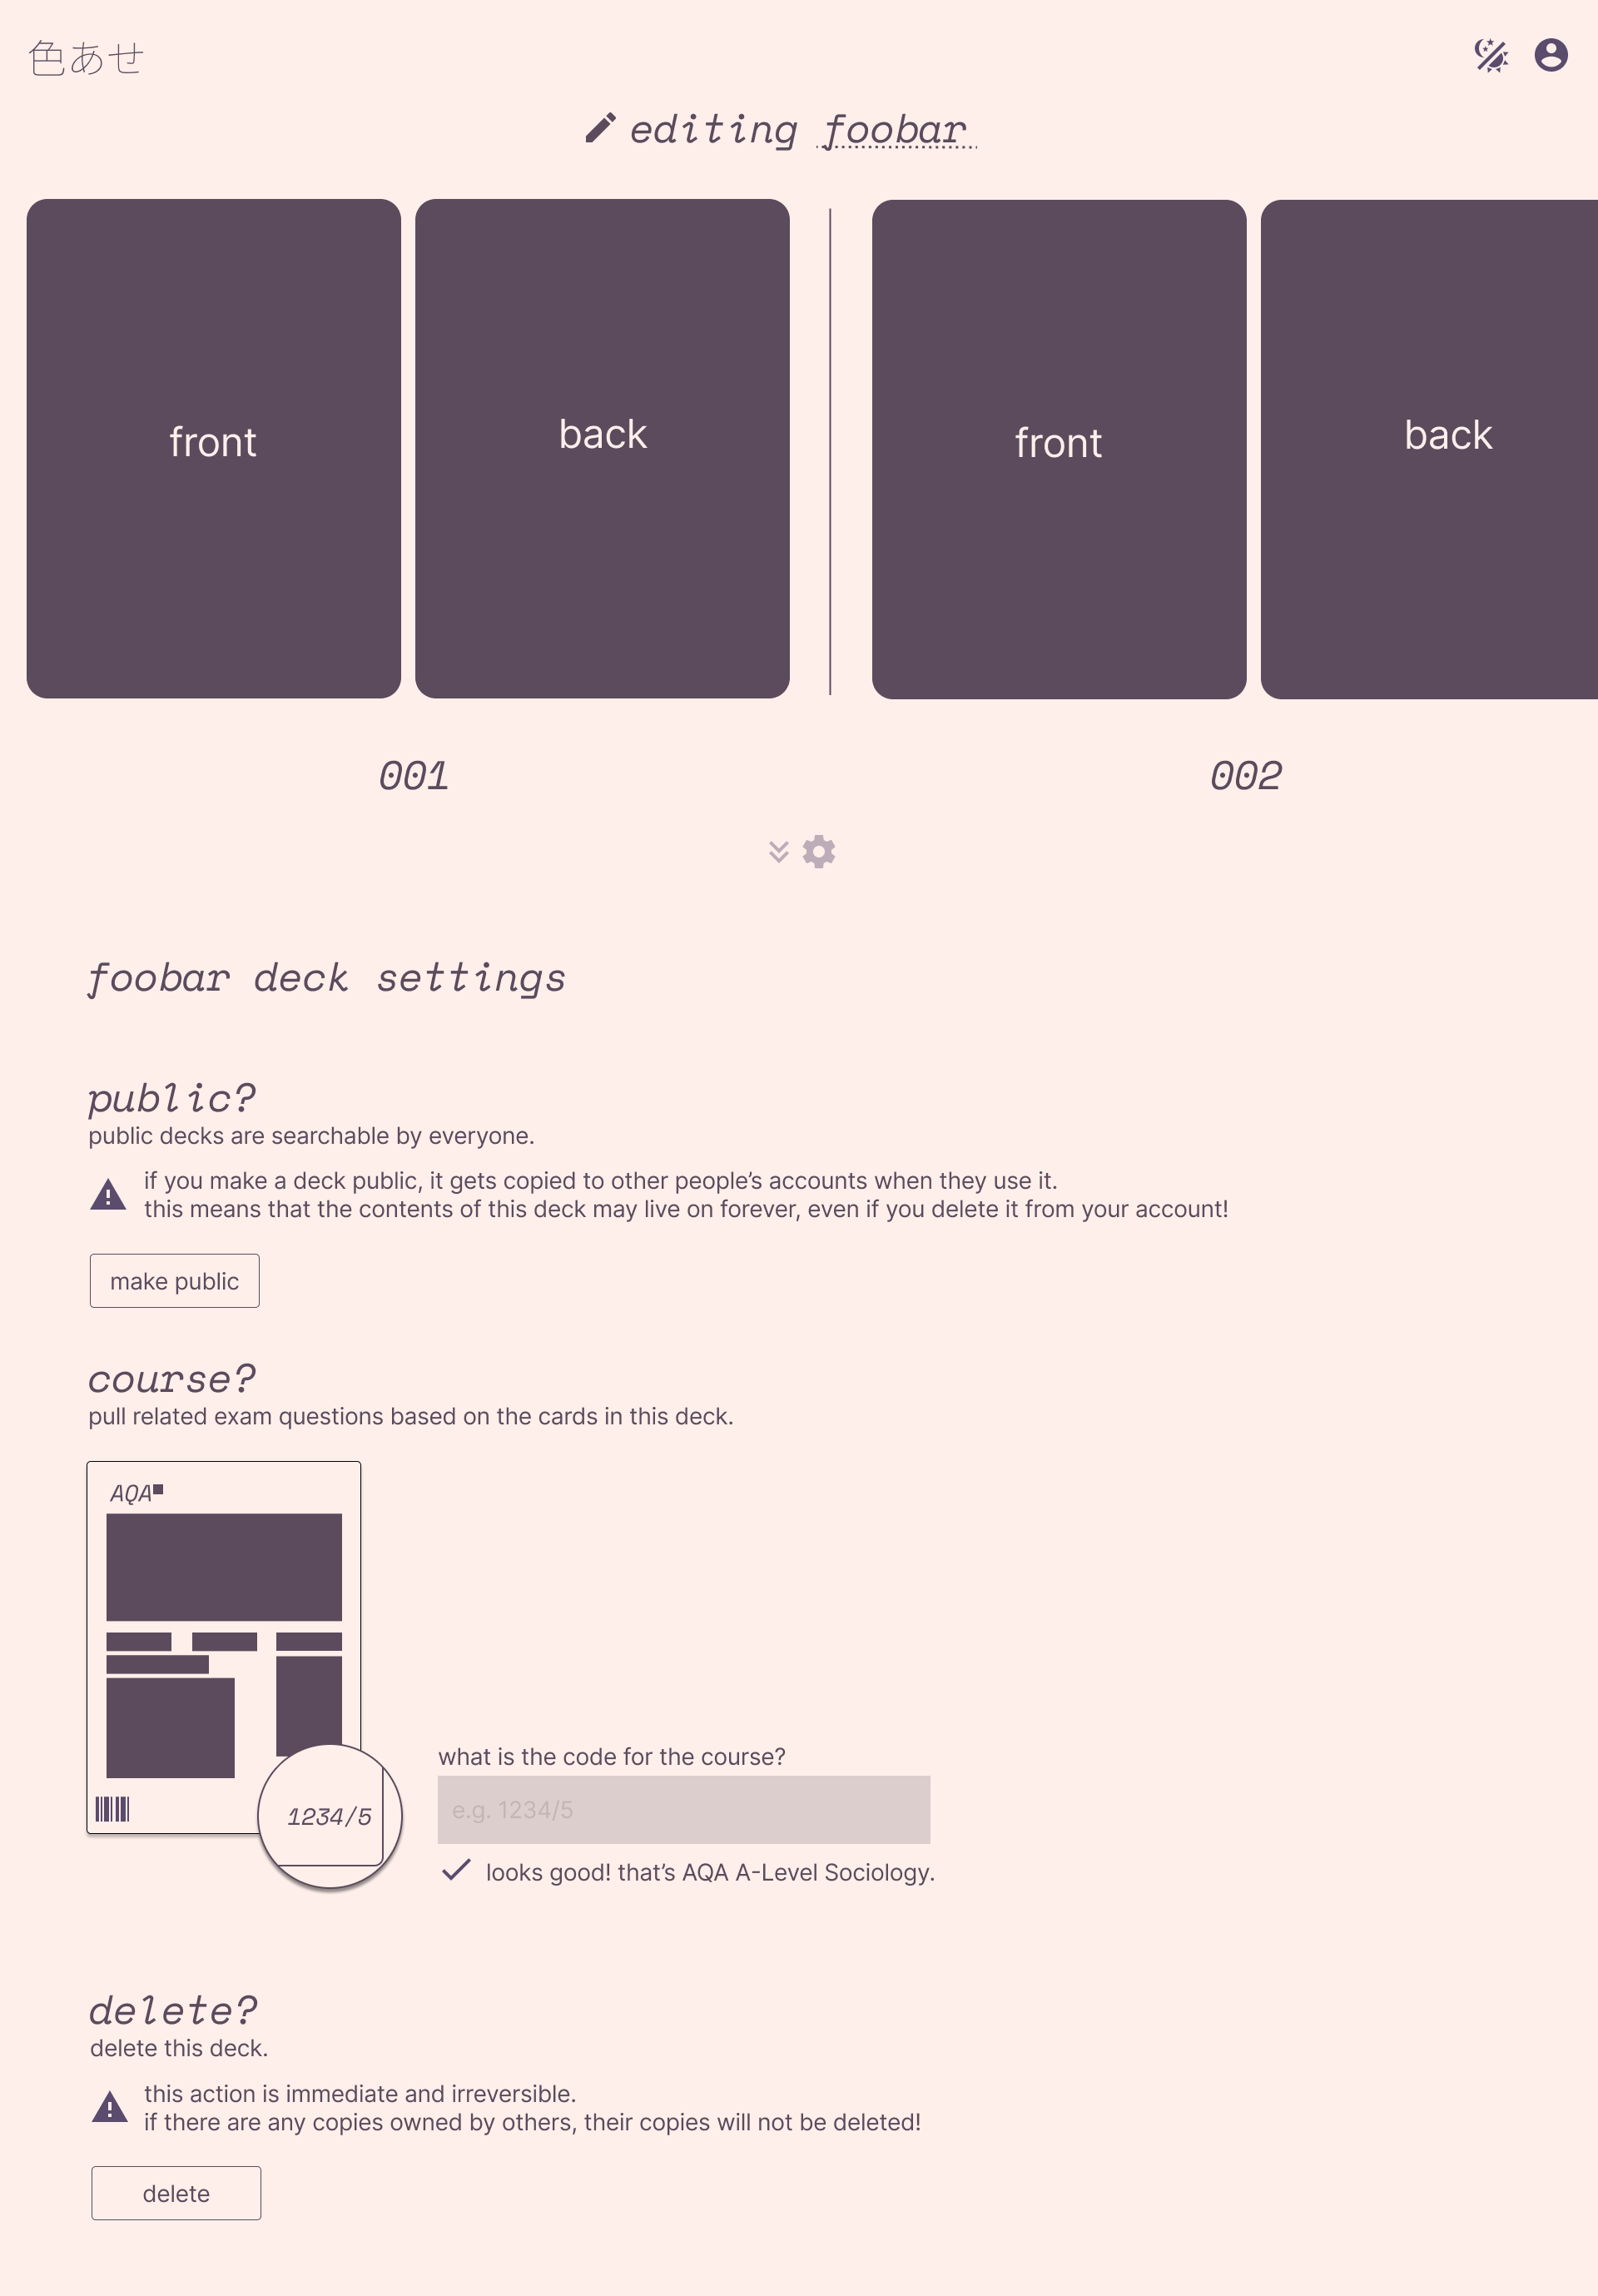
\includegraphics[height=17.5cm]{./media/ui/deck.png}
  \label{fig:editor1}
  \caption{The deck editor. Settings are below the page fold, with a scroll hint telling the user to scroll for settings. They can mark their deck as public, optionally set the course that the deck is related to, or delete the deck. There is a wireframe of the exam paper next to the course box, to assist them in locating the course code. The input box should check to see if the code enters matches a course, and provide feedback.}
\end{figure}

\subsection{Usability}
\subsubsection{Keyboard input}
\paragraph{}
Everything should be accessible via the keyboard. For flipping cards, the user could hit the space bar. For rating cards or picking the correct card from a multiple choice selection, the user should use the number keys for the corresponding item. This makes the interface usable in a highly efficient way, while also being accessible to users who might be blind or lack the motor skills to use a mouse.

\subsubsection{Localisation}
\paragraph{}
While the software will likely be mainly used by those who speak English, we can widen the audience globally by having the interface be translated to many languages. Translators can submit translations by submitting a pull request for their language to the repository; unfortunately, I can't translate the interface myself to other languages.

\subsubsection{Accessibility}
All text in the interface is at a readable size (14px at minimum), and the contrast ratios for text with this colour scheme pass WCAG AA guidelines. The colours that have been chosen should not pose any confusion for people with colour blindness; this has been verified by putting the screens through a colour-blind simulating filter. Touch targets are at least 48px by 48px in size to make them easy to hit.

\section{Testing strategy}
\paragraph{}
A test-driven driven development approach is highly useful. We can designate behaviour that we expect, and then we can iterate solutions very quickly with confidence that the software works as expected. As such, a high quality test suite and plan is essential.

\subsection{TypeScript}
\paragraph{}
TypeScript significantly reduces the amount of tests that need to be written. The TypeScript compiler will detect type issues at compile time, unlike JavaScript, where you are silently left with undefined values at runtime. This means that we don't need to test how functions handle illegal inputs; we can use TypeScript's type system to do this for us, so long as we provide robust type definitions and attach interfaces (a way to define expected types in each field) to our objects.

\subsection{API}
\paragraph{}
Using Jest, we can write tests that specify the behaviour that we want and then expect certain values. We can mock calls to the database to ensure that we have a consistent database state for each test. Each function should be tested with legal inputs (TypeScript's compiler can handle illegal inputs), and each HTTP endpoint should also be simulated by the test library with a range of potential valid and invalid inputs, as would be expected in the real world.

\subsection{End-to-end testing}
\paragraph{}
At the end of development, we can emulate how a real user will interact with the app, from sign up to using cards, using a library such as Cypress to simulate a browser.

\paragraph{}
However, there will still be blind spots in the app that we may have forgotten about. As such, we should give the software to real people and let them use the site, and have them try to break it. There are also some things that need to be tested that simply can't be automated, such as UX. For this, real world usage is vital.

\subsection{Frontend}
\paragraph{}
We can use Google's Lighthouse to identify potential accessibility and performance issues. Lighthouse can flag any issues we need to rectify as well as provide metrics to improve on, such as page load time. We can also simulate a browser using Cypress to test if each component works as expected. However, this also needs to be tested manually by users as not every user action be anticipated.

\chapter{Development}
For the sake of brevity, only the minimum to demonstrate the "idea" of the code is shown in this document. The source code for this project can be viewed \href{https://github.com/iroase-app}{on GitHub, inside the orginsation "iroase-app"} under the BSD-3-Clause license.

\section{Backend}
\paragraph{}
Our stack for the backend is TypeScript, running inside Node, which stores data in a PostgreSQL database. An agile, test-driven development approach is used, with our tests written using \href{https://jestjs.io}{Jest}.

\subsection{Database setup}
The following SQL commands set up our user and session tables in PostgreSQL as according to \hyperref[fig:database1]{our schema}.

\begin{minted}[breaklines, linenos]{sql}
  CREATE TABLE IF NOT EXISTS users (
    "user_id" INT GENERATED ALWAYS AS IDENTITY,
    username varchar NOT NULL,
    hashed_password varchar NOT NULL,
    created timestamp NOT NULL,
    is_moderator boolean NOT NULL DEFAULT false,
    CONSTRAINT users_pk PRIMARY KEY ("user_id"),
    CONSTRAINT users_un UNIQUE (username)
  );

  CREATE TABLE IF NOT EXISTS sessions (
    "session_id" INT GENERATED ALWAYS AS IDENTITY,
    "token" varchar NOT NULL,
    device varchar NOT NULL,
    created timestamp NOT NULL,
    "user_id" INT NOT NULL,
    CONSTRAINT sessions_pk PRIMARY KEY ("session_id"),
    CONSTRAINT "user_id" FOREIGN KEY ("user_id") REFERENCES users("user_id") ON DELETE CASCADE
  );
  );
  
\end{minted}

\subsection{Registration}
\subsubsection{Test cases}

\begin{minted}[breaklines, linenos]{typescript}
// Excerpt from ./src/__test__/register.test.ts
import app from '../app';
describe('/register', () => {
  it('accepts a username and a password and sends back token', async () => {
    const res = await supertest(app)
      .post('/register')
      .send({
        username: 'Fo0bar',
        password: 'secure password',
      });
    expect(res.body).toHaveProperty('session');
    expect(res.body.username).toEqual('foobar');
    expect(res.statusCode).toEqual(201);
  });
  // The full test suite can be found in the repository in the listed file.
});
\end{minted}

\paragraph{}
The server should reject the request if either the "username" or "password" field is missing; the username contains illegal characters; or the username or password is too long or short. "supertest" is a library that makes it easy to emulate a request to an Express web server. The test suite emulates several requests to "/register", and then expects certain responses based on the input it gave the server.

\subsubsection{Implementation}

\begin{minted}[breaklines, linenos]{typescript}
// Excerpt from ./src/api/register/register.ts
register.post('/', async (req, res) => {
  if (!(req.body.username.length && req.body.password.length)) res.status(400).send({ error: 'fieldMissing' });
  else if (!req.body.username.match(/^[A-Za-z0-9]*$/g)) res.status(400).send({ error: 'illegalCharacters' });
  else if (req.body.username.length > 24) res.status(400).send({ error: 'usernameTooLong' });
  else if (req.body.username.length < 3) res.status(400).send({ error: 'usernameTooShort' });
  else if (req.body.password.length > 128) res.status(400).send({ error: 'passwordTooLong' });
  else if (req.body.password.length < 8) res.status(400).send({ error: 'passwordTooShort' });
  else {
    const client = await db.connect();
    try {
      await client.query('BEGIN');
      const user = await client.query(`
      INSERT INTO users (username, hashed_password, created, is_moderator) 
      VALUES ($1, $2, $3, $4) 
      RETURNING user_id;
      `,
      [req.body.username, await argon2.hash(req.body.password), new Date(), false]);

      const token = (await randomBytesP(64)).toString('hex');
      await client.query(`
      INSERT INTO sessions ("user_id", "token", device, created)
      VALUES ($1, $2, $3, $4);
      `,
      [user.rows[0].user_id, token, `${req.useragent?.os}: ${req.useragent?.browser}`, new Date()]);

      await client.query('COMMIT');

      res.status(201).send({ session: token, username: req.body.username });
    } catch (e) {
      if (e instanceof DatabaseError && e.code === '23505') res.status(409).send({ error: 'usernameCollision' });
      else {
        res.status(500).send({ error: 'internalError' });
        console.error(`DB failure!! \n${e}`);
      }
      await client.query('ROLLBACK');
    } finally {
      client.release();
    }
  }
});

\end{minted}

\paragraph{}
We've now checked that the input we get from client requests is what we expect it to be, and then reject any requests that aren't allowed. Next, we attempt to store the user in the database. If the database rejects the operation, we check to see if it was due to a username collision. If so, we notify the client. Finally, for good requests, we send back a session token. We can verify this by running our test suite:

\begin{figure}[h!]
  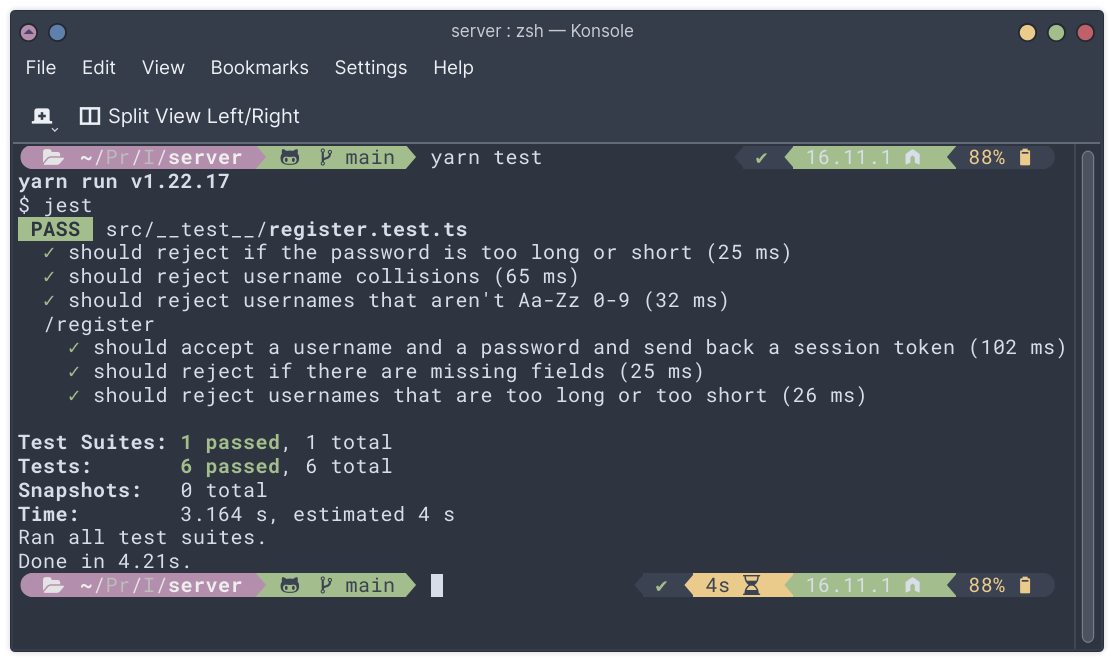
\includegraphics[width=\linewidth]{./media/development/backend/tests/register/pass.png}
  \label{fig:registerValid1}
  \caption{The tests for our registration endpoint pass!}
\end{figure}

\subsection{Making our tests and app containerised}
\paragraph{}
Before we go any further, it's probably wise to make sure that our app and tests run portably. Right now, the test suite (and deployment!) relies on a brittle, manual setup of a database running on the local machine. We can automate our tests and deploys in a reproducible way using Docker. Our \href{https://github.com/iroase-app/server/blob/main/Dockerfile}{Dockerfile} sets out how we should build the Docker image for our server, and our \href{https://github.com/iroase-app/server/blob/main/docker-compose.test.yml}{docker-compose} files show how the image should be deployed alongside a database.

\begin{figure}[H]
  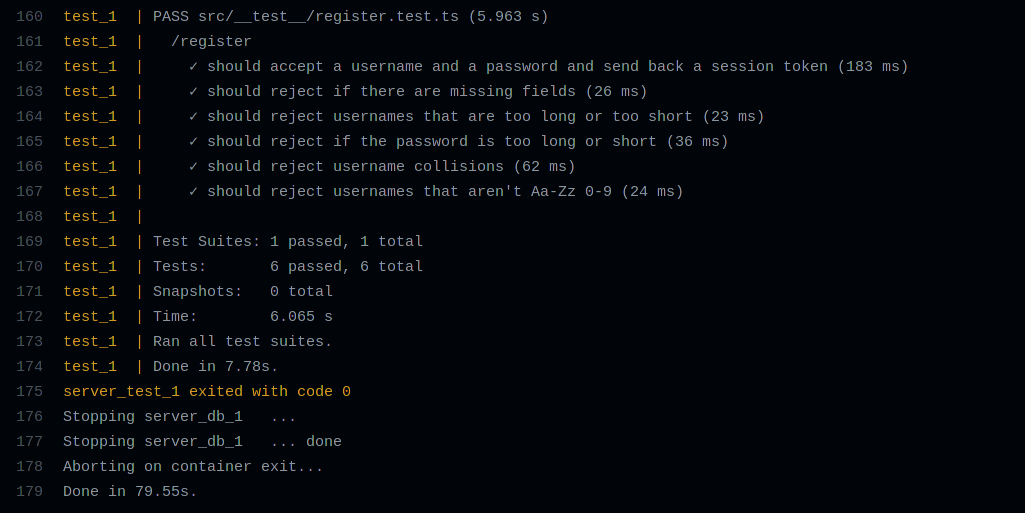
\includegraphics[width=\linewidth]{./media/development/backend/tests/docker/pass.png}
  \label{fig:tests2}
  \caption{We can now run our tests in a continuous integration (CI) environment! Here, the tests are running in GitHub Actions against a clean database.}
\end{figure}

\printbibliography
\end{document}
